\chapter{Implementation Plan and Status}
In this chapter explain the implementation plan and current status of the project along with Ghantt Chart.
	
\section{Latex Help}

\subsection{Tables in Latex}
The investigation utilized the publicly available Credit Card Fraud Detection dataset from Kaggle, containing transactions made by European cardholders in September 2013. Key dataset characteristics are summarized in Table \ref{tab:dataset_stats}.

\begin{table}[h!]
\centering
\caption{Dataset Characteristics and Statistics}
\label{tab:dataset_stats}
\begin{tabular}{lcc}
\toprule
\textbf{Parameter} & \textbf{Value} & \textbf{Percentage} \\
\midrule
Total Transactions & 284,807 & 100\% \\
Fraudulent Transactions & 492 & 0.172\% \\
Legitimate Transactions & 284,315 & 99.828\% \\
Features & 30 & - \\
Time Range & 2 days & - \\
\bottomrule
\end{tabular}
\end{table}

\subsection{Images in Latex}

The dataset contains 28 principal components obtained from PCA transformation, along with 'Time' and 'Amount' features. Figure \ref{fig:feature_dist} shows the distribution of selected features.

\begin{figure}[h!]
\centering
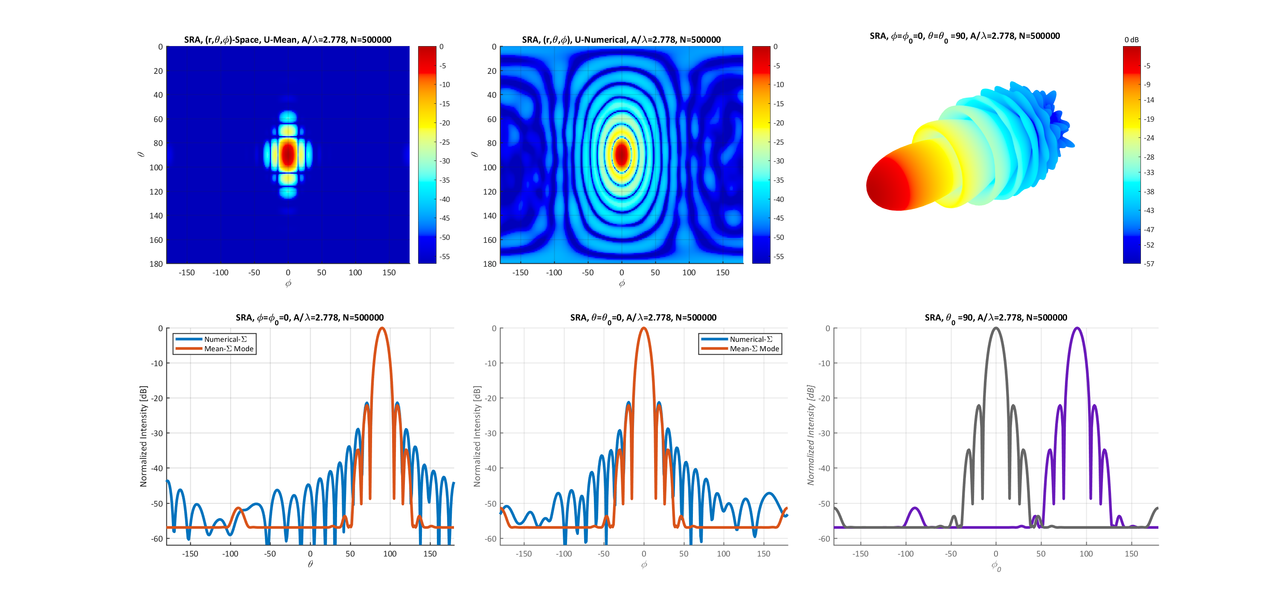
\includegraphics[width=0.8\textwidth]{images/feature_distribution.png}
\caption{Distribution of Features V1, V2, and Transaction Amount}
\label{fig:feature_dist}
\end{figure}



\subsection{List Items in Latex}

Three machine learning algorithms were implemented and compared:

\begin{itemize}
\item \textbf{Random Forest}: Ensemble learning method using multiple decision trees
\item \textbf{Logistic Regression}: Statistical model for binary classification
\item \textbf{Neural Network}: Deep learning approach with multiple hidden layers
\end{itemize}

Numbered:

\begin{enumerate}
	\item \textbf{Random Forest}: Ensemble learning method using multiple decision trees
	\item \textbf{Logistic Regression}: Statistical model for binary classification
	\item \textbf{Neural Network}: Deep learning approach with multiple hidden layers
\end{enumerate}

Nested List:

\begin{enumerate}
	\item Fruits
	\begin{itemize}
		\item Apple
		\item Banana
	\end{itemize}
	\item Vegetables
	\begin{itemize}
		\item Carrot
		\item Spinach
	\end{itemize}
\end{enumerate}


\subsection{Equations in Latex}

Sample Equationslike \eqref{eq:einstein} and \eqref{eq:einstein2}:

\begin{equation}
\text{Normalized Amount} = \frac{\text{Amount} - \mu_{\text{Amount}}}{\sigma_{\text{Amount}}}
\label{eq:einstein}
\end{equation}

\begin{equation}
\text{Time Feature} = \cos\left(2\pi \times \frac{\text{Time}}{86400}\right)
\label{eq:einstein2}
\end{equation}




\subsection{Include Graphics in PDF format}

You can include pdf diagrams for better clarity and printing \ref{fig:roc_curves}.

\begin{figure}[h!]
\centering
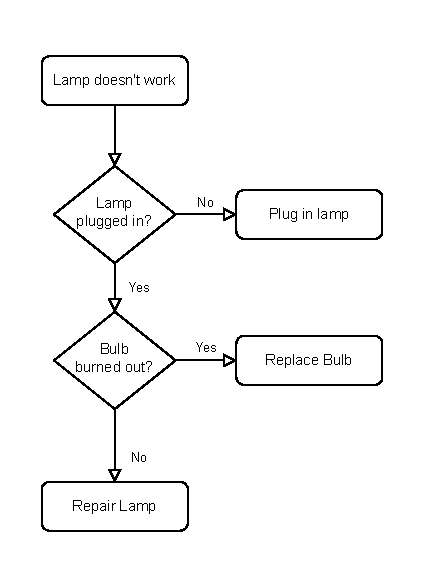
\includegraphics[width=0.8\textwidth]{images/flow.pdf}
\caption{ROC Curves Comparison of Implemented Algorithms}
\label{fig:roc_curves}
\end{figure}

